\documentclass[10pt, a5paper] \url{article}
\usepackage{pdfpages}
\usepackage{parallel}
\usepackage[T2A]{fontenc}
\usepackage{ucs}
\usepackage[utf8x]{inputenc}
\usepackage[polish,english,russian]{babel}
\usepackage{hyperref}
\usepackage{rotating}
\usepackage[inner=2cm,top=1.8cm,outer=2cm,bottom=2.3cm,nohead]{geometry}
\usepackage{listings}
\usepackage{graphicx}
\usepackage{wrapfig}
\usepackage{longtable}
\usepackage{indentfirst}
\usepackage{array}
\newcolumntype{P}[1]{>{\raggedright\arraybackslash}p{#1}}
\frenchspacing
\usepackage{fixltx2e} %text sub- and superscripts
\usepackage{icomma} % коскі ў матэматычным рэжыме
\PreloadUnicodePage{4}

\newcommand{\longpage}{\enlargethispage{\baselineskip}}
\newcommand{\shortpage}{\enlargethispage{-\baselineskip}}

\def\switchlang#1{\expandafter\csname switchlang#1\endcsname}
\def\switchlangbe{
\let\saverefname=\refname%
\def\refname{Літаратура}%
\def\figurename{Іл.}%
}
\def\switchlangen{
\let\saverefname=\refname%
\def\refname{References}%
\def\figurename{Fig.}%
}
\def\switchlangru{
\let\saverefname=\refname%
\let\savefigurename=\figurename%
\def\refname{Литература}%
\def\figurename{Рис.}%
}

\hyphenation{admi-ni-stra-tive}
\hyphenation{ex-pe-ri-ence}
\hyphenation{fle-xi-bi-li-ty}
\hyphenation{Py-thon}
\hyphenation{ma-the-ma-ti-cal}
\hyphenation{re-ported}
\hyphenation{imp-le-menta-tions}
\hyphenation{pro-vides}
\hyphenation{en-gi-neering}
\hyphenation{com-pa-ti-bi-li-ty}
\hyphenation{im-pos-sible}
\hyphenation{desk-top}
\hyphenation{elec-tro-nic}
\hyphenation{com-pa-ny}
\hyphenation{de-ve-lop-ment}
\hyphenation{de-ve-loping}
\hyphenation{de-ve-lop}
\hyphenation{da-ta-ba-se}
\hyphenation{plat-forms}
\hyphenation{or-ga-ni-za-tion}
\hyphenation{pro-gramming}
\hyphenation{in-stru-ments}
\hyphenation{Li-nux}
\hyphenation{sour-ce}
\hyphenation{en-vi-ron-ment}
\hyphenation{Te-le-pathy}
\hyphenation{Li-nux-ov-ka}
\hyphenation{Open-BSD}
\hyphenation{Free-BSD}
\hyphenation{men-ti-on-ed}
\hyphenation{app-li-ca-tion}

\def\progref!#1!{\texttt{#1}}
\renewcommand{\arraystretch}{2} %Іначай формулы ў матрыцы зліпаюцца з лініямі
\usepackage{array}

\def\interview #1 (#2), #3, #4, #5\par{

\section[#1, #3, #4]{#1 -- #3, #4}
\def\qname{LVEE}
\def\aname{#1}
\def\q ##1\par{{\noindent \bf \qname: ##1 }\par}
\def\a{{\noindent \bf \aname: } \def\qname{L}\def\aname{#2}}
}

\def\interview* #1 (#2), #3, #4, #5\par{

\section*{#1\\{\small\rm #3, #4. #5}}

\def\qname{LVEE}
\def\aname{#1}
\def\q ##1\par{{\noindent \bf \qname: ##1 }\par}
\def\a{{\noindent \bf \aname: } \def\qname{L}\def\aname{#2}}
}

\switchlang{ru}
\begin{document}
\title{Использование открытых исходных кодов для разработки 3D сканера и соответствующего программного обеспечения для 3D реконструкции моделей.}
\author{Лина Ширяева, Минск, Belarus \footnote{\url{linashiryaeva@gmail.com}, \url {https://lvee.org/ru/abstracts/257}}}
\maketitle
\begin{abstract}
Nowadays 3D scanning is widely used in different areas of activity. We developed 3D scanner and software using opensource code and open technologies. Using this scanner you can reconstruct models, which size is until 3 metres, with accuracy about 1 mm.   
\end{abstract}
\subsection*{Введение и предпосылки}

В настоящее время 3D-сканирование используется \linebreak в различных сферах деятельности, таких как инженерный анализ, промышленный дизайн, цифровое архивирование, развлечение и игры, медицина и ортопедия и др. Множество конструкций современных 3D-сканеров можно разделить на два типа: лазерные и оптические. На текущий момент существуют свободные аппаратные реализации как лазерных~\cite{Shiryaeva-1}, так и оптических~\cite{Shiryaeva-2} 3D-сканеров. Однако  нам довелось познакомиться с 3D-сканированием поближе при решении достаточно специфической задачи ~--- в ходе разработки оптического 3D-сканера с возможностью сканирования объектов размерами до 3 метров, в связи с чем существующие свободные решения в их исходном виде были неприменимы.

При реализации проекта ставились следующие основные цели: относительно невысокая стоимость сканера, высокая скорость 3D-сканирования и реконструкции, использование открытых источников (исходные коды, библиотеки, SDK) для создания программного обеспечения управления 3D-сканером и работы с 3D-моделями.

\subsection*{Выбор метода 3D-реконструкции}

Задача 3D-реконструкции объекта заключается в определении координат точек объекта в трехмерном пространстве ~--- то есть в получении облака точек объекта. Существует множество различных технологий построения оптических 3D-сканеров: например, камера и поворотный стол~\cite{Shiryaeva-3}, различное количество камер (4 и более, между которыми помещают объект), камера и проектор, и другие. Нами была выбрана открытая технология Structed Light~\cite{Shiryaeva-4} (метод структурной подсветки). В методе структурной подсветки задача реконструкции решается с помощью проектора и камеры: проектор проецирует на объект специальное изображение (структурная подсветка), а фотоаппарат регистрирует объект со специальным изображением (рис. ~\ref{Shiryaeva1}).

\begin{center}
\begin{figure}[h!]
  \centering
  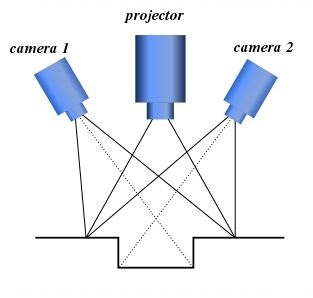
\includegraphics[width=6cm]{Shiryaeva1.jpg}
  \caption{Выбранная конструкция 3D-сканера}
  \label{Shiryaeva1}
\end{figure}
\end{center} 

\subsection*{Подробнее о разработке}

В разработке 3D-сканера, соответствующего ПО к нему и, соответственно, в самом процессе сканирования можно выделить следующие элементы:

\begin{enumerate}
  \item \emph{Конструкция сканера.} В разработанном сканере используются две камеры Canon серии EOS и LCD-проектор разрешением $1920\times1080$ пикселей. Выбранные камеры предоставляют возможность удаленного управления через интерфейс USB. Для написания клиентского приложения, управляющего камерами, использовался родной SDK Canon EOS~\cite{Shiryaeva-5}, реализованный на языке C.
  \item \emph{Калибровка.} Калибровка 3D-сканера состоит из двух этапов: внутренней калибровки отдельных частей сканера, в результате которой рассчитываются фокусные расстояния и дисторсии камер и проектора, и внешней или геометрической калибровки установки, в результате которой мы получаем матрицы поворота и смещения для сопоставления системы координат проектора и камеры. Самым распространенным и простым способом калибровки камеры в данный момент считается метод Zhengyou Zhang~\cite{Shiryaeva-6}, основанный на использовании плоского шаблона в виде шахматной доски. Данный метод реализован в открытой библиотеке OpenCV~\cite{Shiryaeva-7},~\cite{Shiryaeva-8}, распространяемой на условиях лицензии BSD (написана  на C/C++, а также имеет биндинги для Python, Java, Ruby, Lua и др. популярных языков).
  \item \emph{Сканирование.} Основным недостатком метода с использованием нескольких камер без проектора является сложность сопоставления точек двух изображений (т.е. определения координат одной и той же точки на одном и втором изображении). Точка должна обладать характерными особенностями, чтобы ее можно было однозначно идентифицировать. В методе структурной подсветки эта проблема решается за счет правильно подобранного проецируемого шаблона – в итоге мы получаем больше точек (в идеале – все освещенные проектором точки объекта) при меньшем количестве изображений. Т.е. основная задача состоит в выборе такого способа подсветки, который позволит однозначно определить, какая точка изображения проектора освещает точку объекта, зарегистрированную камерой. Мы выбрали для исследования серые коды, как более точные для декодирования. На объект проецируются серые коды для вертикальных и горизонтальных линий. В Structed Light есть реализация двух технологий декодирования: ray-ray (пересечение луча камеры и луча проектора) и ray-plane (пересечение луча камеры с плоскостью проектора). К преимуществам метода ray-ray следует отнести более высокую точность реконструкции в сравнении с методом ray-plane за счет использования как вертикальных, так и горизонтальных линий паттернов, что приводит к увеличению времени сканирования.
  \item \emph{3D-реконструкция.} Построение 3D-облака состоит из следующих этапов: декодирование, расчет оптических лучей камеры и проектора (для метода ray-ray) или расчет оптических лучей камеры и плоскости проектора (для метода ray-plane). Координата точки пересечения лучей камеры и проектора (или плоскости проектора) и является искомой координатой точки 3D-облака. Для работы с 3D-облаками используется Point Cloud Library (PCL)~\cite{Shiryaeva-9} ~--- кроссплатформенная открытая библиотека (Linux, MacOS, Windows и Android/IOS), которая также распространяется в условиях лицензии BSD. В данной библиотеке реализованы различные методы обработки 3D-облаков, такие как сглаживание, фильтрация, совмещения облаков и т.д. Данная библиотека позволяет сохранять 3D-облака в общеизвестных форматах (*.ply, *.obj, *.stl). Начиная с версии 1.8.0 PCL поддерживает распараллеливание расчетов некоторых алгоритмов на GPU. Результат 3D-реконструкции представлен на рис. ~\ref{Shiryaeva2}.
\begin{center}
\begin{figure}[h!]
  \centering
  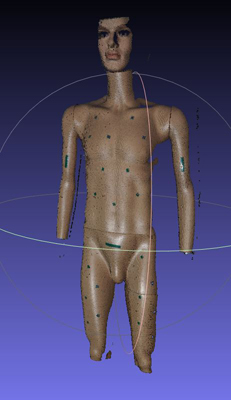
\includegraphics[width=6cm]{Shiryaeva2.jpg}
  \caption{Пример 3D-реконструкции}
  \label{Shiryaeva2}
\end{figure}
\end{center} 
  \item \emph{Построение поверхности.} Облако точек объекта дискретно, и размер точки определяется размером минимально различимого на изображении элемента – пикселя изображения. Чтобы получить данные о всей поверхности объекта, необходимо интерполировать пространство между точками некими поверхностями или функцией. В случае больших и сложных объектов интерполяция одной функцией невозможна. Поэтому обычно применяется интерполяция набором геометрических фигур – «кусочков» плоскостей. Самый простой способ – интерполяция треугольниками (триангуляция). Три точки треугольника однозначно определяют плоскость в пространстве. Для создания триангуляции мы использовали программу с открытым исходным кодом MeshLab~\cite{Shiryaeva-10}. Данная программа распространяется под лицензией GPLv2, имеет реализацию под Linux, Windows и MacOS и предоставляет большой функционал по обработке 3D-облаков и поверхностей.
\end{enumerate}

\subsection*{Заключение}

В заключении хотелось отметить, что использованные особенности конструкции и описанные программные компоненты позволилил создать  3D-сканер с высокой высокой точностью реконструкции (относительная погрешность порядка 1 мм), быстрой скоростью съемки и обработки данных (менее 1 минуты от начала процесса сканирования до получения результата).

%\subsection*{Источники}
\begin{thebibliography}{20}
\bibitem{Shiryaeva-1} \url{http://www.instructables.com/id/DIY-Arduino-3D-Laser-Scanner/}
\bibitem{Shiryaeva-2} \url{http://www.makerscanner.com/docs/1-makerscanner.html}
\bibitem{Shiryaeva-3} \url{http://photopizza.ru/}
\bibitem{Shiryaeva-4} \url{http://mesh.brown.edu/byo3d/source.html}
\bibitem{Shiryaeva-5} \url{https://www.developersupport.canon.com}
\bibitem{Shiryaeva-6} \url{https://www.microsoft.com/en-us/research/wp-content/uploads/2016/02/tr98-71.pdf}
\bibitem{Shiryaeva-7} \url{http://opencv.org}
\bibitem{Shiryaeva-8} \url{http://docs.opencv.org/2.4/doc/tutorials/calib3d/camera\_calibration/camera\_calibration.html}
\bibitem{Shiryaeva-9} \url{http://pointclouds.org/}
\bibitem{Shiryaeva-10} \url{http://www.meshlab.net/\#description}
\end{thebibliography}
\end{document}
